\chapter{Background}
\label{chaBackground}
This chapter gives a brief introduction to programming languages and programming language theory -- though not nearly as comprehensive as a good book on the subject. Typechecking and type inference is also discussed. A birdseye view of computer-hardware and FPGA design is also given, for example what exactly is meant by wordlength.

% Programming languages in general is considered one of the more mature topics in computer science. There are many, many books and papers written on compilers. Some programmars even consider compilers to be black boxes which they must obey, frightened of the complexities and details of the black magic working inside. This background aims to unbox these beasts called compilers and shed some light on them. Explaining all the details of a compiler and the type checker is out of scope for this background.
% 
% Wordlengths, HDLs and also get a section describing how they fit into this work.

\section{Spade}
Spade is a HDL taking a lot of inspiration from Rust to create a more modern HDL (Hardware Description Language). Spade has syntax which mimics that of Rust and tries to remove problems people have when using other HDLs like System Verilog. One of the biggest features of Spade is the static typechecking which allows programs to be verified before even being synthesized -- creating a faster iteration loop.
\cite{src:spadeSomething} \cite{src:spadeAnHDL}

\subsection{Swim}
The Spade-language has a build-tool call Swim. Swim orchestrates things like running PNR, running synthesis tools, installing dependencies, generating basic projects and compiling Spade-code. Swim is the best way to handle any Spade project.

\subsection{Rust}
Rust is a statically typed general purpose systems programming language. The language has recently seen a lot of popularity and boasts features like high performance, reliable software and increased developer productivity. It is also the language that is used to write the Spade compiler and snippets of Rust-code are shown in this work. \cite{src:Rust}

\subsection{The Spade Typechecker}
\todo{Mention ConstraintExpr and Requirements and how constraints are discarded. BitsToRepresent}

\subsection{How Spade Handles Wordlengths}
\todo{}

\subsection{HIR-lowering}
\todo{}

\section{Introduction to Compiler Structure}
What constitutes a compiler is not always obvious. A compiler, in the most banal sense, takes an input program and outputs an output program. Some want the output to be ``simpler`` than the input, passing in a high level program in C and outputting executable X86 machine code where X86 is considered a ``simpler`` than C. The input to the compiler is often text, and we will assume this for the rest of this short introduction to compilers.

Each compiler is unique, but they often have a shared structure. The first step is often to do lexical analysis (also called lexing) in a lexer or tokenizer. Here characters are abstracted away, and the compiler has done the first processing of the text. When lexing the compiler often decide what piece of text is an integer-constant, a keyword, a string, etc. After the lexing the tokens are used to perform syntactic analysis -- also known as parsing. During parsing the compiler understands structures in the program such as what is part of each function or correctly parsing the order of operations for mathematical expressions. The parsing usually produces an abstract syntax tree (AST). Though some compilers interweave these steps, they are usually there in spirit.

The Spade compiler has both a lexer step and a parser step which are located in different modules.

The compilers work is not done yet. After all the syntactical analysis the semantic analysis can be started, semantic analysis is sometimes referred to as the ``inner layers of the compiler``. Here the compiler resolve identifiers, run type-checking and other static program analysis or do optimizations like moving around constants to avoid needless copies. The wordlength inference and optimizations will be an inner layer, the relevant details will be discussed in the Section \ref{sec:TypeChecking}. 

After the compiler has finished optimizing, the output is generated and potentially lowered (made less complex) in multiple stages, often by translating to a simpler internal representation which in the end makes generating the final output of the compiler easier.

One ``layer`` is often called a ``pass``. Spade is a multi-pass compiler and perform these steps sequentially -- there are multiple passes in the Spade compiler.
\cite{src:DragonBook}\cite{src:CraftingInterp}\cite{src:KKLectures}

\begin{figure}
\begin{center}
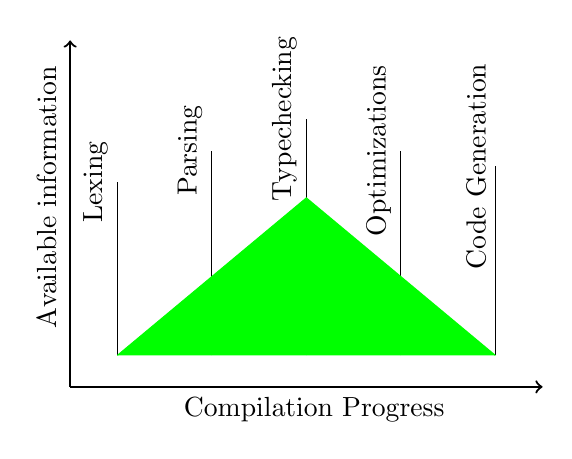
\begin{tikzpicture}[xscale=3, yscale=2]
\draw[->, thick] (-0.2,-0.2) -- (-0.2,2.0) node[xshift=-0.3cm, yshift=-0.2cm, left, rotate=90] {Available information};
\draw[->, thick] (-0.2,-0.2) -- (1.8,-0.2) node[xshift=-2.9cm, below] {Compilation Progress};
\draw (0.0,0) -- (0.0,1.1) node[above, rotate=90] {Lexing};
\draw (0.4,0) -- (0.4,1.3) node[above, rotate=90] {Parsing};
\draw (0.8,0) -- (0.8,1.5) node[above, rotate=90] {Typechecking};
\draw (1.2,0) -- (1.2,1.3) node[above, rotate=90] {Optimizations};
\draw (1.6,0) -- (1.6,1.2) node[above, rotate=90] {Code Generation};
% horizontal line
\filldraw[color=green, fill=green] (0,0) -- (0.8,1.0) -- (1.6,0);
\end{tikzpicture}
  \caption{A visualization of the rough measurement of information present in each step of the compilation process. Typechecking having the most information and lexing and code generation having the least amount of information.}
  \label{fig:InformationCompilation}
\end{center}
\end{figure}

Compilers have to construct a lot of complex information about the program. A visual some find helpful when reasoning about compilers is an imagined graph of ``available information``. Figure \ref{fig:InformationCompilation} tries to communicate the amount of information created in each step of compilation. The most important part being that we know a lot about the program in the type checking phase -- more than when doing syntactical analysis.

\subsection{Abstract Syntax Tree}
General purpose programming languages need to be recursive in their structure -- one might want a sub-expression inside another expression for example. Representing this structure inside a computer cannot simply be done with a simple list of values, the data-structures themselves must reflect the structure of the language. One very popular way of storing this recursive syntactical information is by using an abstract syntax tree (often referred to as an AST). An AST describes the structure of the program.


\begin{figure}
\centering
\begin{subfigure}{.5\textwidth}
  \begin{minted}[]{bnf}
<expr> ::= <num> | <expr> + <expr>

<num>  ::= 1 | 2 | 3
\end{minted}
\end{subfigure}
  \cprotect\caption{A simple grammar for integer expressions. Here an \verb|<expr>| is either a \verb|<num>|, so a simple number, or the it is a sum of 2 \verb|<expr>|.}
  \label{fig:bnfExpr}
\end{figure}
For example, consider the grammar for integer addition expressions described in grammar shown in Figure \ref{fig:bnfExpr}. The syntax understands whole numbers from 1 to 3 and the basic arithmetic operation addition (\verb!+!). Most notable is that the syntax is recursive and expressions can contain expressions in themselves. This BNF-like syntax is a bit simplified and the grammar is not necessarily in a good format. A better grammar would handle order of operations and avoid ambiguities -- which will be explained later.

The basic idea of the BNF is that we can expand each node -- and all expansions are valid ''programs'' in the language. Here valid means syntactically correct -- it does not mean the ideas expressed in the ''program'' are meaningful in any way. The rules expressed in the BNF say that an \verb|<expr>| might be replaced with either \verb|<num>| or \verb|<expr> + <expr>| And that a \verb|<num>| can be replaced with \verb|1| or \verb|2| or \verb|3|. All valid programs are \verb|<expr>| we can start expanding from there -- the simplest program might be \verb|1| since we can get this from expanding \verb|<expr> -> <num> -> 1|. But we could also do the expansions \verb|<expr> -> <expr> + <expr> -> <expr> + <expr> + <expr> -> <expr> + <expr> + <num> -> <expr> + <expr> + 1 -> <expr> + <num> + 1 -> <expr> + 2 + 1 -> <num> + 2 + 1 -> 3 + 2 + 1|. These expansions can get quite repetitive so special notation is often used to abbreviate. This syntax is also so simple that the format expressed here is needlessly powerful. But the important detail here is that we do not know if we expand the left-most \verb|<expr>| or the right more \verb|<expr>| when we apply the rule \verb|<expr> ::= <expr> + <expr>|. To learn more we recommend any book on theoretical computer science. 

We can write a simple ''program'' that is a part of the language described by Figure \ref{fig:bnfExpr}. Some small valid ''programs'' are: \verb!1!, and \verb!1 + 1!. But we will focus on the expression \verb!1 + 2 + 3! -- which has two additions.

Looking at the expression \verb!1 + 2 + 3! it is obvious that the expressions should evaluate to 6. What is not obvious is how a computer should evaluate this expression. We can namely construct two different abstract syntax trees (and two different parse trees) for the program \verb!1 + 2 + 3!. When parsing the program to a syntax tree we have to make the conscious decisions of what node is placed on top.


\begin{figure}
\centering
\begin{subfigure}{.5\textwidth}
\centering
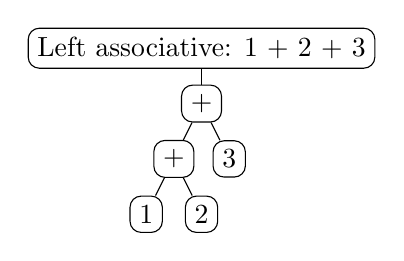
\begin{tikzpicture}[
  sibling distance=2em,
  level distance=2em,
  every node/.style = {shape=rectangle, rounded corners, draw, align=center}
]
  \node {Left associative: 1 + 2 + 3}
          child {node {+}
            child {node {+}
              child {node {1}}
              child {node {2}}
            }
            child {node {3}}
          };
\end{tikzpicture}
\end{subfigure}%
\begin{subfigure}{.5\textwidth}
\centering
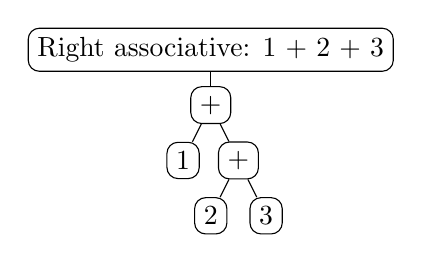
\begin{tikzpicture}[
  sibling distance=2em,
  level distance=2em,
  every node/.style = {shape=rectangle, rounded corners, draw, align=center}
]
  \node {Right associative: 1 + 2 + 3}
          child {node {+}
            child {node {1}}
            child {node {+}
              child {node {2}}
              child {node {3}}
            }
          };
\end{tikzpicture}
\end{subfigure}
  \caption{Two example syntax tree -- illustrating ambiguity in the grammar and the difference between left and right associativity.}
  \label{fig:astExpr}
\end{figure}

The Figure \ref{fig:astExpr} shows the two different associativities that causes \verb!1 + 2 + 3! to be interpreted as either \verb!(1 + (2 + 3))! or \verb!((1 + 2) + 3)!. There is not much difference between these mathematical expressions -- they are even considered equivalent since addition is associative for integers. The associativity property is unfortunately very rare in the real world of effectful-programming. If evaluating an expression in this language had side-effects -- for example printing the result, different associativities would cause different outputs. One of the programs would print \verb+1 2 3 3 6+ while the other would print \verb+1 2 3 5 6+ (ofcourse dependent on how the expressions are evaluated). This is what is called an ambiguity -- and an abstract syntax tree makes it clear how the compiler internally understands this addition.

Making additions have side-effects is not the only way to get non-associative additions, one could use a less well-behaved addition like that found in the IEEE floating point standard -- since any form of rounding is non-associative. Unfortunately infinite precision is quite rare when storage is finite.

There are different operations which can be done to an abstract syntax tree. In our very simple example of integer additions it would make sense to fold the constants and replace the entire AST with the constant 6 -- but to do that we would have to know the associativity of the \verb!+!-operator.

Because of its flexibility the AST is very a very popular format to output from the parsing stage. In the Spade-compiler the AST is annotated with type information as it is discovered -- this annotated AST is then feed either to a language server or a code generation phase.

\section{Type Checking} % Maybe `inner layers`?
\label{sec:TypeChecking}
Type checking is a way of making sure the program is internally consistent -- there are no contradictions inside to program to the program itself. Type checking can be done in different ways with different pros, cons or preferences \cite{src:TypeCheckersBook}. The type checker in Spade can infer types and deduce things about the program, like ``the first argument is a 3-bit integer value, but you gave an enum`` \cite{src:spadeAnHDL}.

The type checker in Spade is a Damas-Hindley-Milner typechecker \cite{src:DamasHindleyMilner}. This means it stops on the first error and can deduce types to their most general form. So if asked to type check the identity function (a function that takes one value and returns the value as is, the function does nothing) the type checker would be able to deduce that the argument could have any type, but that the type is the same as the return value, without any help from the programmar except the body of the function. \cite{src:DamasHindleyMilner}

There is also a connected topic of type inference -- a program that guesses the types of expressions based on the context. A sufficiently good typeinferer could be used to check the types of the program and can easily be modded into a typechecker. It is infact upon this idea that the Damas-Hindley-Milner typechecker works. In this work, we consider typechecking and typeinference the same operations -- since Spade implements typechecking using typeinference. This equivalence is not the same for all typecheckers, since some only check types without inferring.

\subsection{Unification}
A Damas-Hindley-Milner typechecker is a very simple typechecker and is based upon one simple idea: typeinference is a constraint satisfaction problem with \textit{only} equivalence-constraints. The idea of the typechecking and typeinference is to simply find types that has to be equal for the program to function. Most of these small rules are painfully simple -- like: ''adding two numbers gives you a number'', or ''calling a function results in a type with the return value of the called function''. What really drives these simple rules is a process called unification. Unification is a way to propagate these equality constraints. This is proven to be correct, given that all expressions without sub-expressions have a type.

This unification property is also found in logic-programming, which is not a coincidence but rather an effect of the Curry–Howard isomorphism. \cite{src:curryHowardIso}

We find examples useful to quickly get basic understanding of a topic, so we will outline the typechecking of a simple program and how the unification step would work. We will typecheck the simple program in Figure \ref{fig:progUni}.

\begin{figure}
\centering
\begin{subfigure}{.5\textwidth}
  \begin{minted}[linenos]{rust}
fn add<A> : (A, A) -> A

fn main { add(add(1, 2), "abc") }
\end{minted}
  \end{subfigure}
  \caption{A simple dummy program to show unification. A simple ''add'' function is defined which takes 2 arguments of the same type and returns that type. Types are denoted with uppercase letters and language constructs are defined using lowercase letters.}
  \label{fig:progUni}
\end{figure}

\begin{figure}
\centering
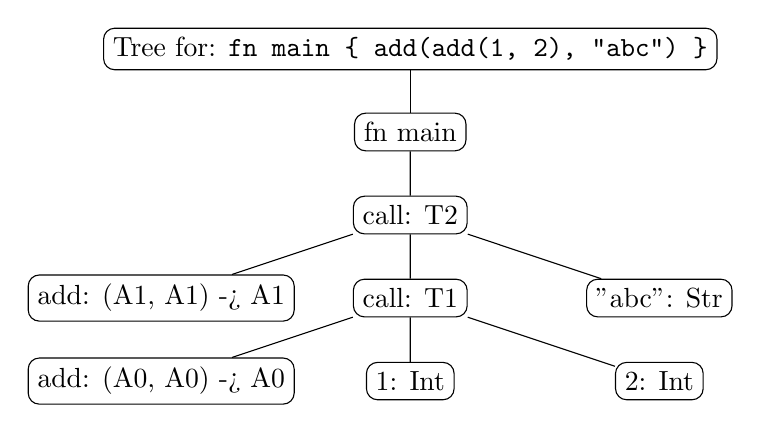
\begin{tikzpicture}[
  sibling distance=9em,
  level distance=3em,
  every node/.style = {shape=rectangle, rounded corners, draw, align=center}
]
  \node {Tree for: \verb|fn main { add(add(1, 2), "abc") }|}
          child {node {fn main}
              child {node {call: T2}
                    child {node {add: (A1, A1) -> A1}}
                    child {node {call: T1}
                        child {node {add: (A0, A0) -> A0}}
                        child {node {1: Int}}
                        child {node {2: Int}}
                    }
                    child {node {"abc": Str}}
              }
          };
\end{tikzpicture}
  \cprotect\caption{The syntax tree for \verb|fn main { add(add(1, 2), "abc") }| with the generated type variables before we have annotated all the types.}
  \label{fig:progUniTree}
\end{figure}

\begin{figure}
\centering
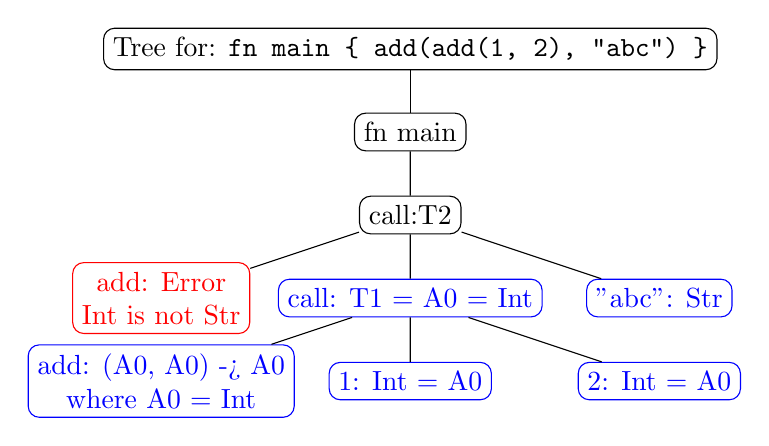
\begin{tikzpicture}[
  sibling distance=9em,
  level distance=3em,
  every node/.style = {shape=rectangle, rounded corners, draw, align=center}
]
  \node {Tree for: \verb|fn main { add(add(1, 2), "abc") }|}
          child {node {fn main}
              child {node {call:T2}
                    child {node[color=red] {add: Error\\Int is not Str}}
                    child {node[color=blue] {call: T1 = A0 = Int}
                        child {node[color=blue] {add: (A0, A0) -> A0\\where A0 = Int}}
                        child {node[color=blue] {1: Int = A0}}
                        child {node[color=blue] {2: Int = A0}}
                    }
                    child {node[color=blue] {"abc": Str}}
              }
          };
\end{tikzpicture}
  \cprotect\caption{The syntax tree for \verb|fn main { add(add(1, 2), "abc") }| with the generated type variables after we have inferred as far as we can. We see an error marked in red and finished nodes which are marked in blue. The error was found when we tried to unify \verb|Str| with \verb|Int| since the call requires both arguments to be the same type.}
  \label{fig:progUniTreeAfter}
\end{figure}


Let us assume that we have two types in our language \verb+Int+ and \verb+Str+. We start by giving each construction a unique type variable. (The unique type variable is mainly to aid explanation. There are more resource efficient ways of implementing Damas-Hindley-Milner.) We then evaluate the syntax tree bottom up -- the syntax tree is shown in Figure \ref{fig:progUniTree}. We will also assume the rules: 
\begin{enumerate}
  \item integer-constants have the type \verb+Int+
  \item String-constants have the type \verb+Str+
  \item Calling a function means the types of the arguments and parameters are the same and the whole expressions evaluates to the return type of the function. Evaluating rule (3) always gives a new type ''A'', we will keep track of these with numbered suffixes.
\end{enumerate}
These 3 simple rules let us typecheck and typeinfer the expression in the main-function.

In this explanation the \verb+:+ operator denotes that an expression on the left has a known type on the right, so \verb+1:Int+ means the expressions \verb+1+ has type \verb+Int+. We will also denote the unifications of types, so \verb+A9=A8+ means the type \verb+A9+ is the same types as \verb+A8+. We first of all know the type of all the simple expressions -- thanks to rules (1) and (2) -- that means \verb+1:Int+, \verb+2:Int+ and \verb+"abc":Str+. We can now solve \verb+add(1, 2)+ by applying rule (3) to \verb+add:(A0, A0) -> A0+ and \verb+add(1, 2):T1+, we can unify \verb+(Int, Int)+ and \verb+(A0, A0)+, which gives \verb+A0=Int+. We also get \verb+T1=A0=Int+ which gives us \verb+add(1, 2):Int+. The more complex expression is now inferable \verb+add(add(1, 2), "abc"):T2+, we unify \verb+(T1, Str)+ and \verb+(A1, A1)+ which gives us a contradiction, since \verb+T1=Int=/=Str+ -- this would result in a type error which might be thrown by the compiler. This result is shown in the Figure \ref{fig:progUniTreeAfter}

In conclusion, unification lets us define two types as the same type and send all this information as far as we want in a program -- there are programming languages with global type-inference for example. But the method described by Damas-Hindley-Milner is limited to equality-constraints which has some limitations in what types can be expressed.

\subsection{Monomorphisation}
After all the typechecking and typeinference has been done monmorphisation can take place. This phase turns generic functions into concrete function -- that is to say all functions with generics like \verb+fn add<A>(x: A, y: A) -> A+ are given concrete types like \verb+fn add(x: i32, y: i32) -> i32+. This means the same code can lead to multiple function bodies. Monomorphisation creates a new instance of a function for each of the generic arguments given, and Rust does something similar. \cite{src:rustMono}

Monomorphisation is often considered a performance optimization, but for HDLs this step is absolutely required since the hardware does not handle function pointers or any kind of indirection. For it to be possible to pass around program code as a concept there would also need to be some kind of control flow structure -- the only control flow structure available on an FPGA is a mask. So modeling virtual methods from object oriented programming would need to be done using masks, this means the resource usage would grow with the number of implementations for a virtual method, since we cannot know at compile time which of these results is the right one (unless we use monomorphisation) -- the scaling of this solution negates all the benefits of virtual methods and is not a good fit for FPGA development where resources are scarce. 

\subsection{The Curry-Howard Isomorphism}
\todo{And why mapping logic systems and type systems between eachother is a good idea}

\subsection{The Lambda Cube}
\todo{Mention Haskell, PureScript and Coq and some about the Lambda Cube}

\section{Interval Arithmetic, Affine Arithmetic and Self Validating Numerical Methods}
\label{sec:IAndAA}

Mathematical expressions are everywhere -- and somehow even more so in computer science since the only thing computers can do is evaluate expressions. What is mainly useful for this work is what is referred to as self validating numerical methods -- these methods give you a way of estimating the potential values of arbitrary mathematical expressions. Two of these methods will be the focus of this work, interval arithmetic (IA) and affine arithmetic (AA). There is an excellent explanation of both IA and AA by \citeauthor{src:affAri}\cite{src:affAri} -- the following section is a short version to cover the absolute basics of the material. This section simplifies away a lot of details when it comes to rounding -- which is crucial if this is to be implemented for anything using floating point numbers -- but since this work is only interested in integers this can be simplified.

Affine arithmetic and interval arithmetic are two common ways to estimate the value of arbitrary mathematical expressions. AA and IA can be applied to estimate bounds for mathematical functions and thus all things that can be modeled by mathematical functions. Since programs can be modeled using mathematical expressions IA and AA have a place in static analysis of programs, which is the focuses of this work. These methods are often referred to as over-estimation or self validating numerical methods.


\subsection{Interval Arithmetic}
Interval arithmetic operates on intervals, as the name implies. A value -- or in the context of a program, a variable -- has a smallest and largest value it can assume. Consider \verb`x = random_real()`, where \verb`random_real` generates a random value in the range $[0, 1]$. We can express this in interval arithmetic as $\bar{x} = [0, 1]$, intervals will be denoted with a bar on top to separate them from the variables. Note especially that the true value of $x$ lies in the interval $\bar{x}$. In this example we know $0 \leq x \leq 1$, also written as $x \in [0, 1]$. These intervals can be added, negated, and so on, to give you an estimate of an arbitrary expression. The empty interval is also defined and written as $[]$. The empty interval usually denotes expressions or code that cannot be reached or evaluated -- it a very sane default value for merging together multiple branchen in a Spade match-statement, since if there are no matches we would infact have unreachable code.

\subsubsection{Interval Arithmetic: An Example and Limitations}
Some of the rules for interval arithmetic are:
\begin{enumerate}
  \item $n * [a, b] = [n * a, n * b]$
  \item $[a, b] - [c, d] = [a - d, b - c])$
  \item $[a, b] + [c, d] = [a + c, b + d]$
\end{enumerate}

We will be using the expression $2x + z - z$ as an example where $x = [0, 1], z = [1, 3]$. This mean we have the expression after expanding the variables which we can calculate:
\begin{align*}
  2x + z - z \\
  =^{\text{expansion}} \quad & 2 * [0, 1] + [1, 3] - [1, 3] \\
  =^{1}                \quad & [2 * 0, 2 * 1] + [1, 3] - [1, 3] \\
  =^{2}                \quad & [0, 2] + [1 - 3, 3 - 1] \\
  =^{\text{simplify}}  \quad & [0, 2] + [-2, 2] \\
  =^{3}                \quad & [0 + -2, 2 + 4] \\
  =^{\text{simplify}}  \quad & [2, 4]
\end{align*}
We start by applying the scaling rule (1) -- then the subtraction rule (2) and last the addition rule (3) giving us $2x + z - z = [-2, 4]$. This means the expression $2x + z - z$ with the context $x = [0, 1], z = [1, 3]$ always lies in the range $[-2, 4]$.
\label{sec:prevResultIA}

The conclusion we've reached is true, but the estimate is larger than it necessarily needs to be. Notice that subtracting the value $z$ from itself should result in $0$, which is a perfectly valid point and correct point. This is a limitation of the interval arithmetic. Interval arithmetic does not reason about the expressions that came before it and how they combine, and this limitation would exist if used to do static analysis of programs. But AA understand the relations between variables we evaluate if we provide the context. AA can more accurately calculate expressions like $a - a$ since it understands that $a$ and $a$ must hold the same value. 

\subsection{Affine Arithmetic}
Affine arithmetic (AA) works similarly to interval arithmetic (IA), but has a memory of where values come from and can reason about their combinations at a higher level. That said, AA does not produce strictly better results than IA in all circumstances. However, the intersection of the results will produce better results than each individually. \cite{src:affAri}

Though affine arithmetic is more sophisticated it does not always produce better results, interval arithmetic can for some computations produce tighter bounds. There are other methods for overestimation that are considered more sophisticated like ME-gPC \cite{src:MEgPC} and modified affine arithmetic, but the extra complexity can be added later if it is found to be needed. ME-gPC was not considered for this work due to its complexity -- but it is a good extension to the techniques explained in this work. Affine arithmetic and interval arithmetic are the simplest methods that offer enough complexity to make this work interesting.

\subsubsection{Affine Arithmetic: An Example and Limitations}
In affine arithmetic there is a concept of noise symbols ($e_i$ where $i$ is a real number between $[-1, 1]$) and the numbers half width ($x_i$ where $i$ is a real number). A linear combination of these noise symbols is a reasonable way to represent a "number" when reasoning about affine arithmetic, $\hat{x} = x_0 + x_1e_1 + x_2e_2 + \dots$. These terms can then be combined using similar rules to interval arithmetic. Notice how the first term lacks a noise symbol, this expresses where the center of the uncertainty is. The different noise variables serve as the memory of this expression, consider subtracting $\hat{x} - \hat{x}$ with itself we get the expected result of 0 from that. \cite{src:affAri} 


Here is an excerpt of relevant rules for affine arithmatic, for our simple example of $2x + z - z$ as an example where $x = [0, 1], z = [1, 3]$.
\begin{enumerate}
  \item $[a, b] \Rightarrow x_0 = (a + b) / 2, x_n = (a - b) / 2$ where $n$ is unique, this maps a range to its affine form $\hat{x}$
  \item $n * \hat{x} = \hat{z}$ where $z_n = n * x_n$
  \item $-\hat{y} = \hat{z}$ where $z_n = -x_n$
  \item $\hat{x} + \hat{y} = \hat{z}$ where $z_n = x_n + y_n$
  \item $\hat{x} \Rightarrow [a, b]$ where $a = \sum{x_ie_i}: e_0 = 1, e_n = -1$ and $b = \sum{x_ie_i}: e_0 = 1, e_n = 1$
\end{enumerate}

We start by expanding the context $x = [0, 1], z = [1, 3]$ from ranges to their affine form using (rule 1), $\hat{x} = 0.5 + 0.5e_x, \hat{z} = 2 + 1e_z$, we can then expand the expression and use our other rules.

\begin{align*}
    2x + z - z \\
    =^{\text{expansion}} \quad & 2 * (0.5 + 0.5e_x) + (2 + e_z) - (2 + e_z) \\
    =^{2} \quad & (1 + e_x) + (2 + e_z) - (2 + e_z) \\
    =^{3} \quad & (1 + e_x) + (2 + e_z) + (-2 + -e_z) \\
    =^{4} \quad & (3 + e_x + e_z) + (-2 + -e_z) \\
    =^{4} \quad & (1 + e_x + 0e_z) \\
    \Rightarrow^{5} \quad & [1 - 1 - 0, 1 + 1 + 0] = [0, 2]\\
\end{align*}

We start by applying the scaling rule (2), then we simplify subtraction to a negation and an additon using rule (3). Now we just have a final summation using rule (4) twice. After all this the expression can be changed to a range using rule (5) which gives us $[0, 2]$, which is exactly $2x$ -- the answer that would have been preferred in Section \ref{sec:prevResultIA}. There is of course nothing magical going on here, all of these calculations are just simple algebra and we could just as easily have expanded the first expressions directly without using any special rules. However, this simplification cannot always be used. 

\subsection{When Interval Arithmetic Is Better Than Affine Arithmetic}
Affine arithmetic may seem like the superior option in all cases -- this is not true. Affine arithmetic has trouble with multiplication, and has to add extra noise in order to constantly overestimate. If we consider the simple case of multiplying two expressions in affine form $a + e_a$ and $b + e_b$ where $e_a$ and $e_b$ are noise variables we can use simple multiplication rules we get $(a + e_a)(b + e_b) = ab + ae_b + be_a + e_ae_b$, this is almost a valid affine form expression. But the pesky $e_ae_b$ term is illegal in AA. Since we have not defined what multiplying noise variables is (this is infact the next improvement we can do and this would get us into ME-gPC) though doing this would require handling squared noise variables which causes other problems which are out of scope. The way \cite{src:affAri} define multiplication is slightly different -- simplified they overestimate using $|(a * b)| \leq |(|b| * a + |a| * b + \text{mid}(a) * \text{mid}(b) + \text{rad}(a) * \text{rad}(b))|$ where ''min'' denotes the picking the value without a noise variable of an affine form and ''rad'' summing all terms which have a noise variable of the affine form. The extra terms are then added to a new noise variable which causes multiplications to become partially opaque -- AA cannot understand the full result of a multiplication. This means any multiplication breaks $a - a = 0$ and adds noise. This noise causes us to increase the radius -- and if the lower limit is something like $0$ which is very special in multiplication we clearly get better results with interval arithmetic.

This extra noise is particularly relevant when handling large expressions. Interval arithmetic can fare a lot better here since multiplication does not add noise in the same way. One very concrete example is if all variables in an expression like $\prod x_i$ are in the range $[0,n)$ -- affine arithmetic does not respect $0$ in the same way and would give us a range poking out below $0$ while interval arithmetic would correctly infer the lower bound of $0$.

When concerned with estimating arithmetic expressions we can both get the pie and eat it. Since both interval arithmetic and affine arithmetic offer estimates which are guaranteed to hold all potential values, we can take the subset of the guesses and still keep correctness.

\section{Wordlength Inference and Typechecking in Spade}
\label{sec:TheProblem}
Most values in Spade take up bits or space in the run time environment. Wordlength inference is mostly concerned with numbers -- so consider positive numbers without a decimal. Consider a program with a counter that resets to 0 after counting to 3, we do not need 32 bits to represent it. The cost of storing a number with 32 bits compared to 2 bits could be large if it requires a larger FPGA, extra circuit components or a different power rating. Compared to software engineering of programs for general purpose computers where memory is considered abundant, FPGAs are limited in memory and computations use parts of the FPGA (which isn't possible on a processor using fixed width numbers) which causes HDLs to be designed differently to a general purpose programming languages.

Wordlength inference is the compiler understanding what wordlength -- the number of bits -- is needed to store a value. Inferring this value well causes good resource usage and requires less manual intervention. Doing it poorly or not at all either requires users to manually specify the wordlength of each value, or hardware that is inefficient.

In Spade integer types are written using the \verb|int| keyword, and wordlength is specified by passing a generic to the integer type. \verb|int<3>| specifies an integer that spans 3 bits and holds values between $-(2^2) = -4$ and $2^2 - 1 = 3$. Spade also infers wordlengths based on the number of additons and multiplications -- so one addition adds one extra bit of required precision while a multiplication adds the wordlengths together. This approach means that equivalent expressions require different wordlengths depending on the number of additions and multiplications used to express it. 

\begin{figure}
\centering
\begin{minted}[linenos]{rust}
fn f(a: int<3>) -> int<4> {
  a + 1 + 1
}

entity main(clk: clock, rst: bool) -> int<4> {
  f(3)
}
\end{minted}
\caption{A simple spade program that does not compile, showing the current limitations of wordlength inference.}
\label{figSimpleFaultSpade}
\end{figure}

\begin{figure}
\centering
  \begin{minted}[]{text}
error: Type error
  |- src/simple\_fault.spade:1:27
  |
1 |   fn f(a: int<3>) -> int<4> {
  |                      ------ int<4> type specified here
  | |---------------------------^
2 | |   a + 1 + 1
3 | | }
  | |-^ Found type int<5>
  |
  = Expected: 4
  =       in: int<4>
  =      Got: 5
  =       in: int<5>

Error: aborting due to previous error
\end{minted}
\caption{The output from the compiler when trying to compile the program in Figure \ref{figSimpleFaultSpade}}
\label{figSimpleFaultSpadeCompileOutput}
\end{figure}

Consider the program in Figure \ref{figSimpleFaultSpade}. The function \textit{f} adds 3 values together, two of which are known constants. We also know that $2^2 + 2 < 2^3$ -- we should be able to fit the result of the addition into the 4 bit word without loss of data. The compiler does not agree as seen in the compiler output in Figure \ref{figSimpleFaultSpadeCompileOutput} where it claims we need 5 bits to store this value. This problem might seem inconsequential since calculating constant expressions during compilation would fix this, as seen by the program in Figure \ref{figSimpleCorrectSpade} compiling without worries. Adding constants is only the top of the iceberg that is this problem. The problem here is much deeper, and is a direct cause of the implementation of typechecking and wordlength inference directly.

\begin{figure}
\centering
  \begin{minted}[linenos]{rust}
fn f(a: int<3>) -> int<4> {
  a + 2
}

entity main(clk: clock, rst: bool) -> int<4> {
  f(3)
}
\end{minted}
  \caption{``simple\_correct.spade`` A spade program that does compile and is equivalent to the program in Figure \ref{figSimpleFaultSpade}}
\label{figSimpleCorrectSpade}
\end{figure}

The Spade compiler implements a Damas-Hindley–Milner typechecker -- discussed in more detail in Section \ref{sec:TypeChecking}. Damas-Hindley-Milner runs in almost linear time (if implemented correctly) but is not complete. The completeness property for type checkers means there are programs which are correct but that the type checker will not recognize as correct. The programs from Figures \ref{figSimpleFaultSpade} and \ref{figSimpleCorrectSpade} are an example of this. This observation is important since it means this is not a bug, but a limitation of the compiler itself.

\section{Field Programmable Gate Array}
A field programmable gate array (FPGA) is an application specific integrated circuit (ASIC). An FPGA is slower and draws more power than a ''normal'' circuit but FPGAs allow very fast iteration since they are programmable and are cheaper to produce in small volumes. This makes FPGAs ideal for prototyping hardware designs. An FPGA is made up of a grid of components all connected by configurable interconnections -- each component can then be programmed and connected individually. \cite{src:FPGA}

An FPGA is very different from a general purpose computer or CPU which is what is mostly programmed by highlevel languages. An FPGA is a circuit which means all steps are taken simultaneously -- this allows massive parallelism. This makes FPGAs ideal for things like realtime signal processing -- which is why they see a lot of use in media processing and military applications \cite{src:FPGAApplications}. These physical limitations also put restrictions on the HDL. This is why variables are immutable in Spade.

\subsection{Synthesis}
Synthesis is a step which tries to simplify the boolean functions that make up a logical circuit and in turn give out logical gates. This is done by analysing the expressions and solving a minimization problem. This process is usually deterministic and is a step that tries to allocate as few gates as possible to build a circuit. In the case of FPGAs synthesis is often results in creating look up tables.

\subsection{Place and Route}
Place and Route, sometimes referred to as PNR in this work is when the program is encoded as hardware and happens after the synthesis step, which requires routing the information in the actual chip and deciding what node is responsible for what computation. This is similar to how the routes are placed on a ''normal'' circuit and is considered a computationally hard problem. Since the problem of PNR is computationally hard, a stochastic algorithm is applied, meaning the same program might not generate identical encoded hardware. When trying to measure the resource usage of FPGA programs this step needs to be run multiple times, since one run could always be a fluke.
